\begin{figure}[htbp]
\section*{ SMARCC2}
\centering
\begin{subfigure}[b]{0.95\textwidth}
\centering
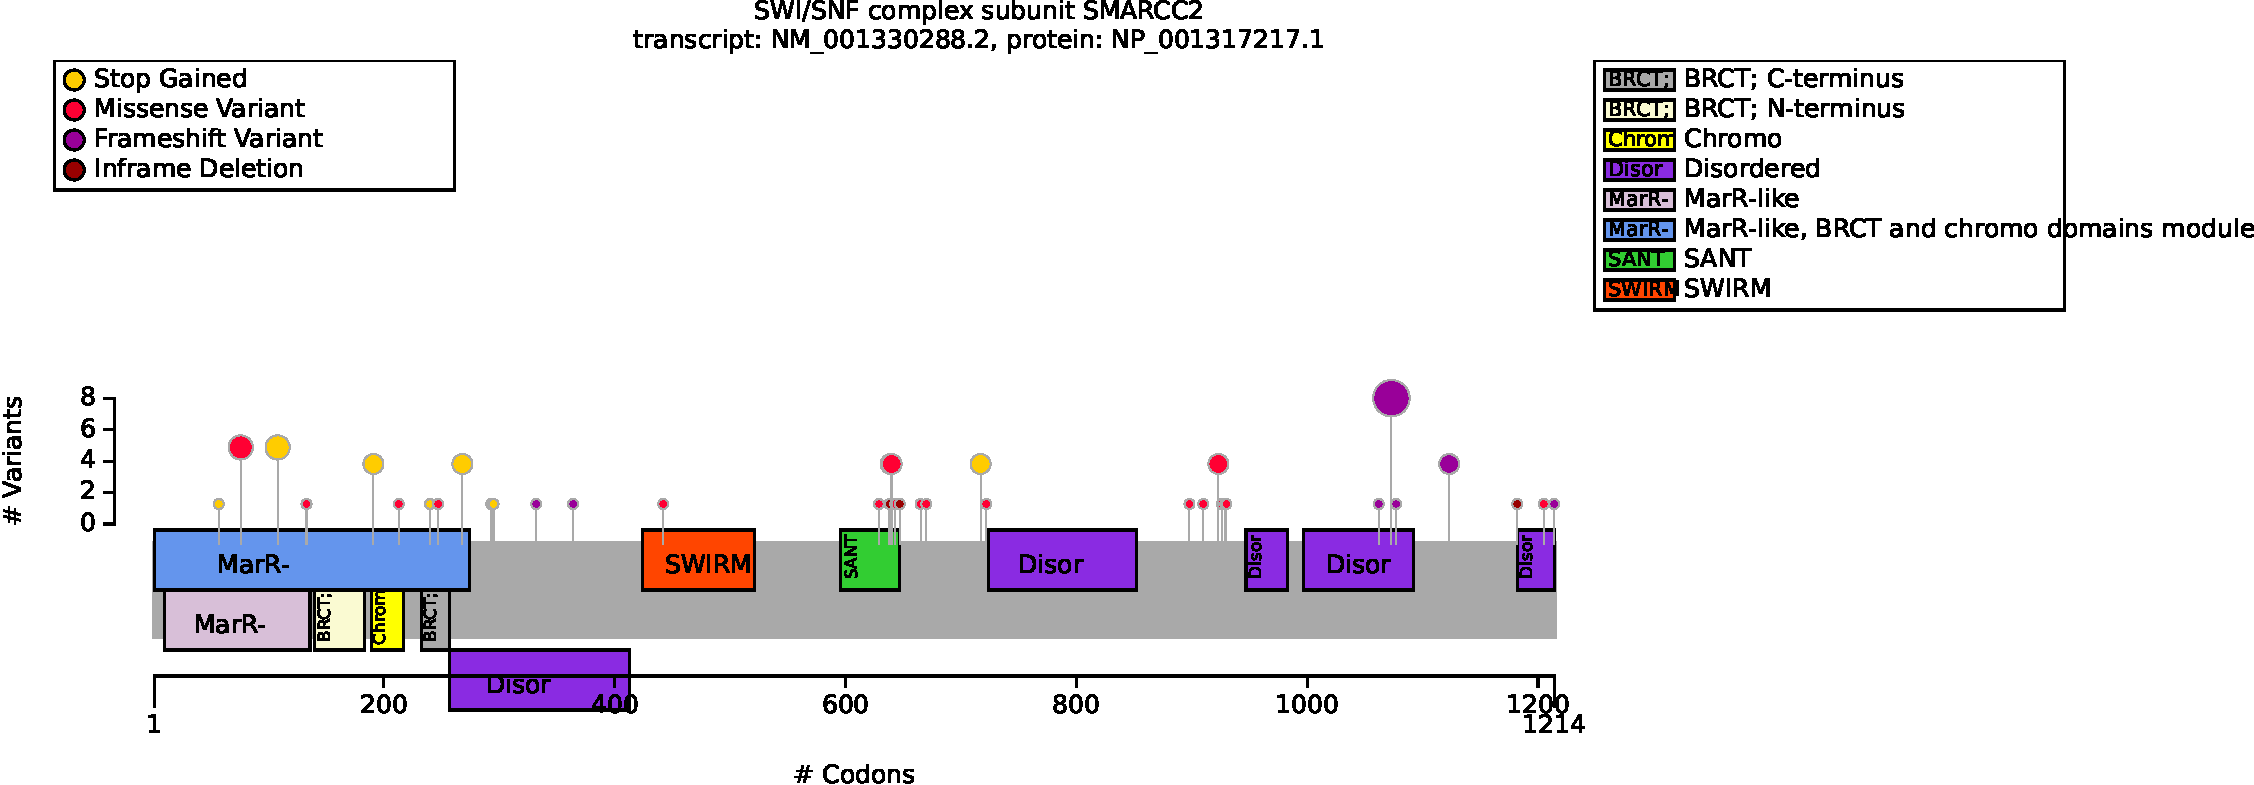
\includegraphics[width=\textwidth]{ img/SMARCC2_protein_diagram.pdf} 
\captionsetup{justification=raggedright,singlelinecheck=false}
\caption{Distribution of variants in SMARCC2}
\end{subfigure}

\vspace{2em}

\begin{subfigure}[b]{0.95\textwidth}
\centering
\resizebox{\textwidth}{!}{
\begin{tabular}{llllrr}
\toprule
HPO term & c.3222del & other & p-value & adj. p-value\\
\midrule
Intellectual disability [HP:0001249] & 1/6 (17\%) & 49/52 (94\%) & $6.99\times 10^{-5}$ & 0.002\\
Autistic behavior [HP:0000729] & 7/8 (88\%) & 13/51 (25\%) & 0.001 & 0.017\\
\bottomrule
\end{tabular}
}
\captionsetup{justification=raggedright,singlelinecheck=false}
\caption{Fisher Exact Test performed to compare HPO annotation frequency with respect to c.3222del and other. Total of
        24 tests were performed.}
\end{subfigure}
\vspace{2em}
\begin{subfigure}[b]{0.95\textwidth}
\centering
\resizebox{\textwidth}{!}{
\begin{tabular}{llllrr}
\toprule
HPO term & N term & Other & p-value & adj. p-value\\
\midrule
Mild global developmental delay [HP:0011342] & 11/15 (73\%) & 10/43 (23\%) & 0.001 & 0.027\\
\bottomrule
\end{tabular}
}
\captionsetup{justification=raggedright,singlelinecheck=false}
\caption{Fisher Exact Test performed to compare HPO annotation frequency with respect to N term and Other. Total of 23 tests were performed.}
\end{subfigure}
\vspace{2em}
\begin{subfigure}[b]{0.95\textwidth}
\centering
\resizebox{\textwidth}{!}{
\begin{tabular}{llllrr}
\toprule
Genotype (A) & Genotype (B) & total tests performed & significant results\\
\midrule
Missense & Other & 23 & 0\\
FEMALE & MALE & 26 & 0\\
\bottomrule
\end{tabular}
}
\captionsetup{justification=raggedright,singlelinecheck=false}
\caption{Fisher Exact Test performed to compare HPO annotation frequency with respect to genotypes.}
\end{subfigure}

\vspace{2em}

\caption{The cohort comprised 65 individuals (24 females, 37 males, 4 with unknown sex). A total of 118 HPO terms were used to annotate the cohort. 
Disease diagnosis: Coffin-Siris syndrome 8 (OMIM:618362). Bosch et al. (2023) reported correlations for  missense versus truncating variant cohorts for 
Global developmental delay; Intellectual disability (HP:0001263;HP:0001249): p = 0.005 (FDR-corr: 0.033); Muscular hypotonia (HP:0001252): p = 0.004 (FDR-corr: 0.033);
mild GDD/ID (HP:0011342;HP:0001256): p = 0.012 (FDR-corr: 0.051); Abnormality of the outer ear (HP:0000356): p = 0.013 (FDR-corr: 0.051); 
Decreased body weight (HP:0004325): p = 0.002 (FDR-corr: 0.024); Abnormality of the eye (HP:0000478): p = 0.000 (FDR-corr: 0.008);
Short stature (HP:0004322): p = 0.006 (FDR-corr: 0.035); Feeding difficulties/failure to thrive (HP:0011968;HP:0001508): p = 0.013 (FDR-corr: 0.051) \cite{PMID_37551667}. 
The authors did not specifically test c.3222del. Differences in results may be due to different assumptions of the analysis procedure. Code to reproduce the results in 
Bosch et al. was not available. A total of 65 unique variant alleles were found in \textit{SMARCC2} (transcript: \texttt{NM\_001330288.2}, protein id: \texttt{NP\_001317217.1}).}
\end{figure}
